\documentclass[signature=data]{physicsreport}
\usepackage{graphicx}

%%
%% User settings
%%

\classno{}
\stuno{}
\groupno{}
\stuname{}
\expdate{\expdatefmt\today}
\expname{分光计的调节和应用}

%%
%% Document body
%%

\begin{document}
% First page
% Some titles and personal information are defined in ``\maketitle''.
\maketitle
% \section{实验目的}
\section{实验预习}
\newpage

\section{实验现象及数据记录}
% Teacher signature
\makeatletter
\physicsreport@body@signature{data}
\makeatother

\newpage

% Data process and others


\section{数据处理}

\begin{enumerate}
    \item 分别计算相应三种颜色的光(绿光、黄光1、黄光2)在衍射级次k=1、2、3时波长的测量值λk,并计算波长平均值$\overline \lambda$,将$\overline \lambda$与汞灯波长的标准值相比较,计算测量的相对误差。要求写出完整的计算过程,包括所用公式和代入实验数据后的表达式。
    \item 计算衍射光栅对黄光1和黄光2在衍射级次k=1、2、3时的角色散率$D_k$。
    \item 计算三棱镜的顶角、绿光对应的最小偏向角,计算三棱镜材料对绿光的折射率,双黄光的折射率测量为选做内容。
\end{enumerate}




\pagebreak
\section{讨论题}

\subsection{应用分光计进行测量之前,应调节到何种状态?}



\subsection{按游标原理,读出下图中的角度数。}

\begin{figure}[H]
    \centering
    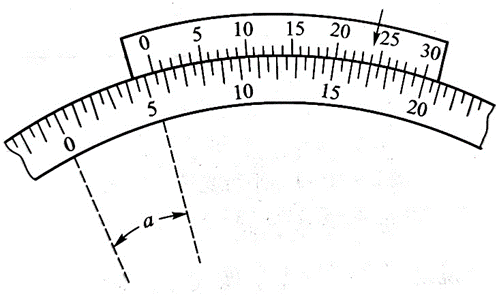
\includegraphics[width=0.5\textwidth]{images/lab13/image.png}
    % \caption{分光计游标读数}
    \label{fig:lab13-fig1}
\end{figure}

\end{document}